\documentclass[a4paper]{jpconf}
\usepackage{graphicx}
\usepackage{hyperref}
\usepackage[activate={true,nocompatibility},final,tracking=true,kerning=true,spacing=nonfrench,factor=1100,stretch=15,shrink=15]{microtype}
\SetTracking{encoding={*}, shape=sc}{0}

\begin{document}
\title{Fast emulation of track reconstruction in the CMS simulation}

\author{Matthias Komm, on behalf of the CMS collaboration}

\address{Centre for Cosmology, Particle Physics and Phenomenology,
Universit\'e catholique de Louvain, Louvain-la-Neuve, BELGIUM}

\ead{Matthias.Komm@cern.ch}

\begin{abstract}
Simulated samples of various physics processes are a key ingredient within analyses to unlock the physics behind LHC collision data. Samples with more and more statistics are required to keep up with the increasing amounts of recorded data. During sample generation, significant computing time is spent on the reconstruction of charged particle tracks from energy deposits which additionally scales with the pileup conditions. In CMS, the FastSimulation package is developed for providing a fast alternative to the standard simulation and reconstruction workflow. It employs various techniques to emulate track reconstruction effects in particle collision events. Several analysis groups in CMS are utilizing the package, in particular those requiring many samples to scan the parameter space of physics models (e.g. SUSY) or for the purpose of estimating systematic uncertainties. The strategies for and recent developments in this emulation are presented, including a novel, flexible implementation of tracking emulation while retaining a sufficient, tuneable accuracy.
\end{abstract}


\section{Introduction}
Tracking of charged particles is one of the crucial ingredients to understand the physics behind LHC collisions. In the CMS experiment~\cite{cms}, tracks of charged particles are reconstructed and matched to information gathered by other subdetectors which improves the overall event reconstruction and resolution~\cite{pf}. From reconstructed tracks higher analysis level objects like jets and the missing transverse energy are derived. 

Sophisticated tracking algorithms are required to reconstruct tracks from the large amount of charged particles transversing the CMS detector at each bunch crossing. A typical instantaneous luminosity of $10^{34}\,\mathrm{cm}^{-2}\mathrm{s}^{-1}$, which was reached in 2016, can lead to more than 500 reconstructed tracks originating from 20--30 proton-proton interactions per crossing.

The complex, multistep algorithms which reconstruct tracks from energy depositions left by traversing charged particles in the CMS tracker are very computing-intense. The standard track reconstruction procedure for data is applied to simulated events as well after they have passed the emulation of the electronic response of the detector. However, at this point in the simulation chain, it can be beneficial to sidestep the standard reconstruction by utilizing truth-information about the simulated events instead. In the CMS simulation framework this idea together with others has led to a fast alternative for simulating physics events called \textsc{FastSimulation}~\cite{fsim1,fsim2}. Such a fast alternative is further motivated in the light of the planned increase of luminosity for which larger samples of simulated events with higher pileup conditions have to be produced.

The goal of the \textsc{FastSimulation} package of CMS, which is tightly integrated into the CMS software~\cite{cmssw}, is to provide a fast alternative to the standard simulation and reconstruction workflow while delivering high-level analysis objects with sufficient accuracy. This is achieved by sidestepping certain parts in the production of simulated event samples to achieve a significant speed up. The two major CPU-intense parts which are replaced are the Geant4-based~\cite{geant4} simulation of particle interactions with the detector material and the track reconstruction. The final analysis objects are indistinguishable from the ones produced by the standard simulation work flow. This enables an easy integration of \textsc{FastSimulation} samples in analyses along samples from the standard simulation and data.

Nowadays, the \textsc{FastSimulation} package is successfully employed within CMS analyses. Typical use cases are searches for beyond the standard model physics such as SUSY. Such analyses require usually multiple signal samples which reflect various realizations of a new physics model. Other use cases are the evaluations of the impact of systematic uncertainties on a measurement like a variation of the renormalization and factorization scales or the top quark mass. A more general use case is to enhance the statistics of existing samples for training multivariate analysis methods.

This article is organized as follows: First, the steps involved in the standard track reconstruction are described briefly. Then, their alternative implementation within the \textsc{FastSimulation} package is detailed with an emphasis on new developments in its tracking emulation. After the validation where the tracking performance of the standard simulation and reconstruction is compared to \textsc{FastSimulation} this article is summarized and an outlook on planned developments is provided.


\section{Standard track reconstruction within CMS}
The standard track reconstruction is applied to real data and to simulated events from the standard Geant4-based simulation. It begins with the forming of hits on the pixel and strip modules of the tracker. Dedicated templates of charge depositions from simulation are compared to data to infer the position of a hit on a pixel module~\cite{pixelav}. On the strip modules, hits are seeded from strips and subsequently combined with adjacent ones if their readout is sufficiently above their noise level.

The reconstructed hits are then passed to the track reconstruction sequence which finds tracks iteratively. After each iteration the hits within the tracks that pass certain quality requirements are masked in next iterations to reduce the combinatorics. Currently, there are eight iterations deployed which will however be adapted after the upgrade of the pixel detector in 2017~\cite{pixelphase1}. The first iterations target easy-identifiable, non-displaced tracks with respect to the interaction region, whereas the later iterations are designed for more complicated situations. Seeds are built from hit doublets or triplets on specific tracker layers which pass an iteration-dependent acceptance selection. Then, trajectories are constructed through the combinatorial track finder~(CTF) algorithm which tries to locate seed-compatible hits on other layers. It is based on Kalman filters and pattern recognition techniques.  Finally, the track parameters are estimated from a fit to the hit positions using a Runge-Kutta-based propagator which accounts for material effects and the inhomogeneous magnetic field. Tracks for analyses have to pass certain quality criteria depending on the iteration to reject ``fake'' tracks from spurious hit combinations. The fake rate is found to be about 5--15\% depending on the momentum and particle type in the standard simulation and reconstruction.

More information on the standard track reconstruction can be found in Ref.~\cite{trackreco}.


\section{Fast emulation of track reconstruction}

In \textsc{FastSimulation}, the simulation of energy loss of particles as they traverse the detector is performed using parameterized probability functions for emulating energy loss through ionization, nuclear scattering, and bremsstrahlung. No detailed information of charge deposition on the pixel and strip modules is generated. To mimic the resolutions of the standard hit reconstruction the true hit positions are smeared. A new \textsc{FastSimulation} module for position smearing was recently developed which allows to manage various algorithms for position smearing side-by-side. It can be flexibly configured for any topology of the tracker. Additionally, each algorithm can be restricted to certain tracker modules only. Currently, a simple Gaussian smearing of the position is deployed for all strip modules where the configured resolution depends on the specific tracker subdetector and its layer. A more detailed emulation of hit reconstruction is employed for the pixel modules where parametrized distributions from the standard template-based hit reconstruction are utilized for the smearing. Furthermore, the new module allows the emulation of merging of two hits which occurs when the distributions of the deposited charge from two transversing particle overlap. Figure~\ref{fig:merge} shows a recent study of the probability of hit merging on the pixel modules. Such probability maps are expected to be used for the emulation of hit merging in the future.

\begin{figure}[htbp]
\begin{center}
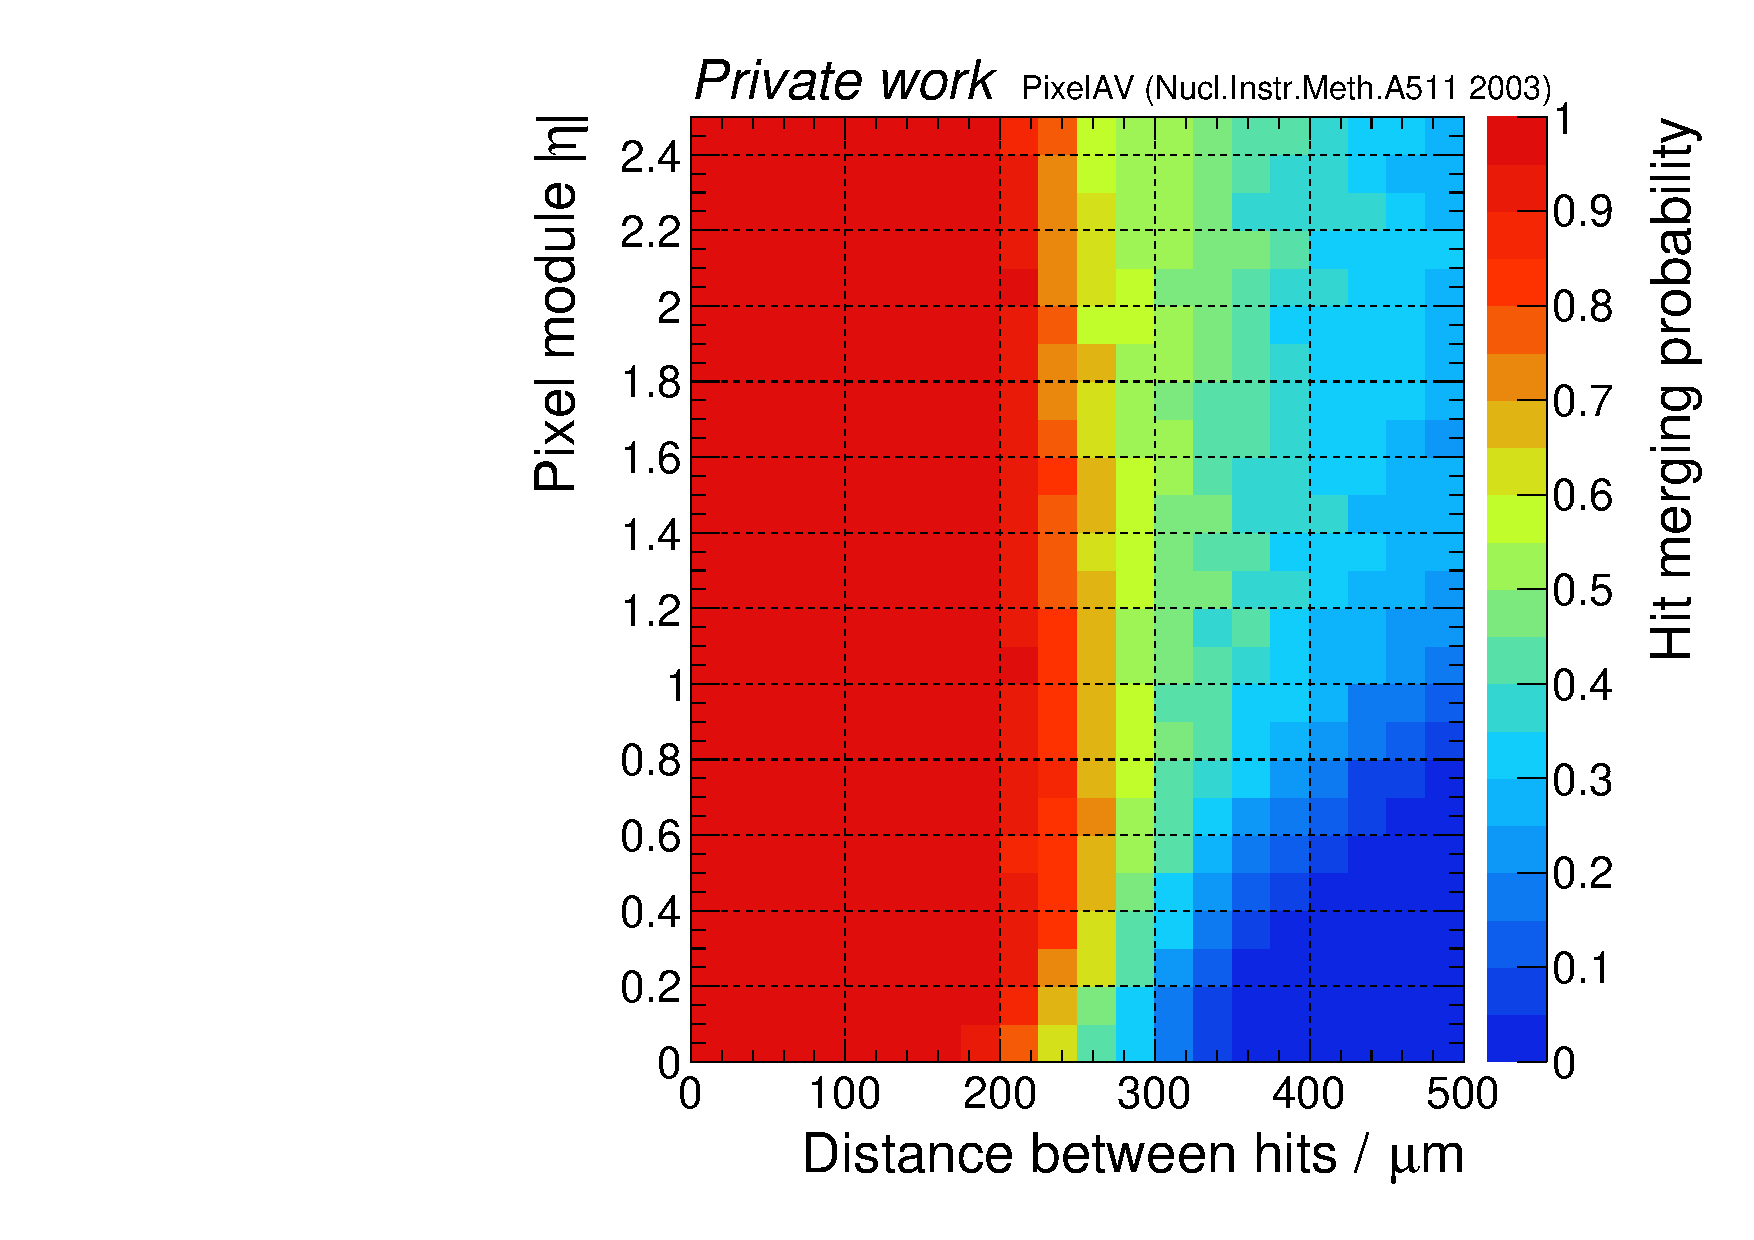
\includegraphics[width=0.4\textwidth]{figures/merge.pdf}
\caption{\label{fig:merge}Probability of two hits merging on the pixel barrel modules as a function of their distance and local incident angle of a track expressed in pseudorapidity.}
\end{center}
\end{figure}

By default, the seeding and trajectory building modules of the standard iterative tracking sequence are replaced completely within \textsc{FastSimulation}. An overview is provided in Fig.~\ref{fig:tracking}. The ability to produce merged hits originating from close particle tracks necessitated a recent refactoring of the \textsc{FastSimulation}-specific data objects within the iterative tracking sequence. As motivated in the introduction, the main idea of sidestepping the reconstruction by using truth information about the origin of each hit remains, but had to be extended. Instead of a one-to-one mapping of reconstructed hits to true particle tracks, close simulated hits can now result into a single reconstructed ``merged'' hit that can be shared between the final tracks within an iteration. A further benefit is that the mapping itself can be generated independently from the truth information which will allow the mix-in of wrong hit combinations leading to ``fake'' tracks in the future which are currently not emulated.

\begin{figure}[htbp]
\begin{center}
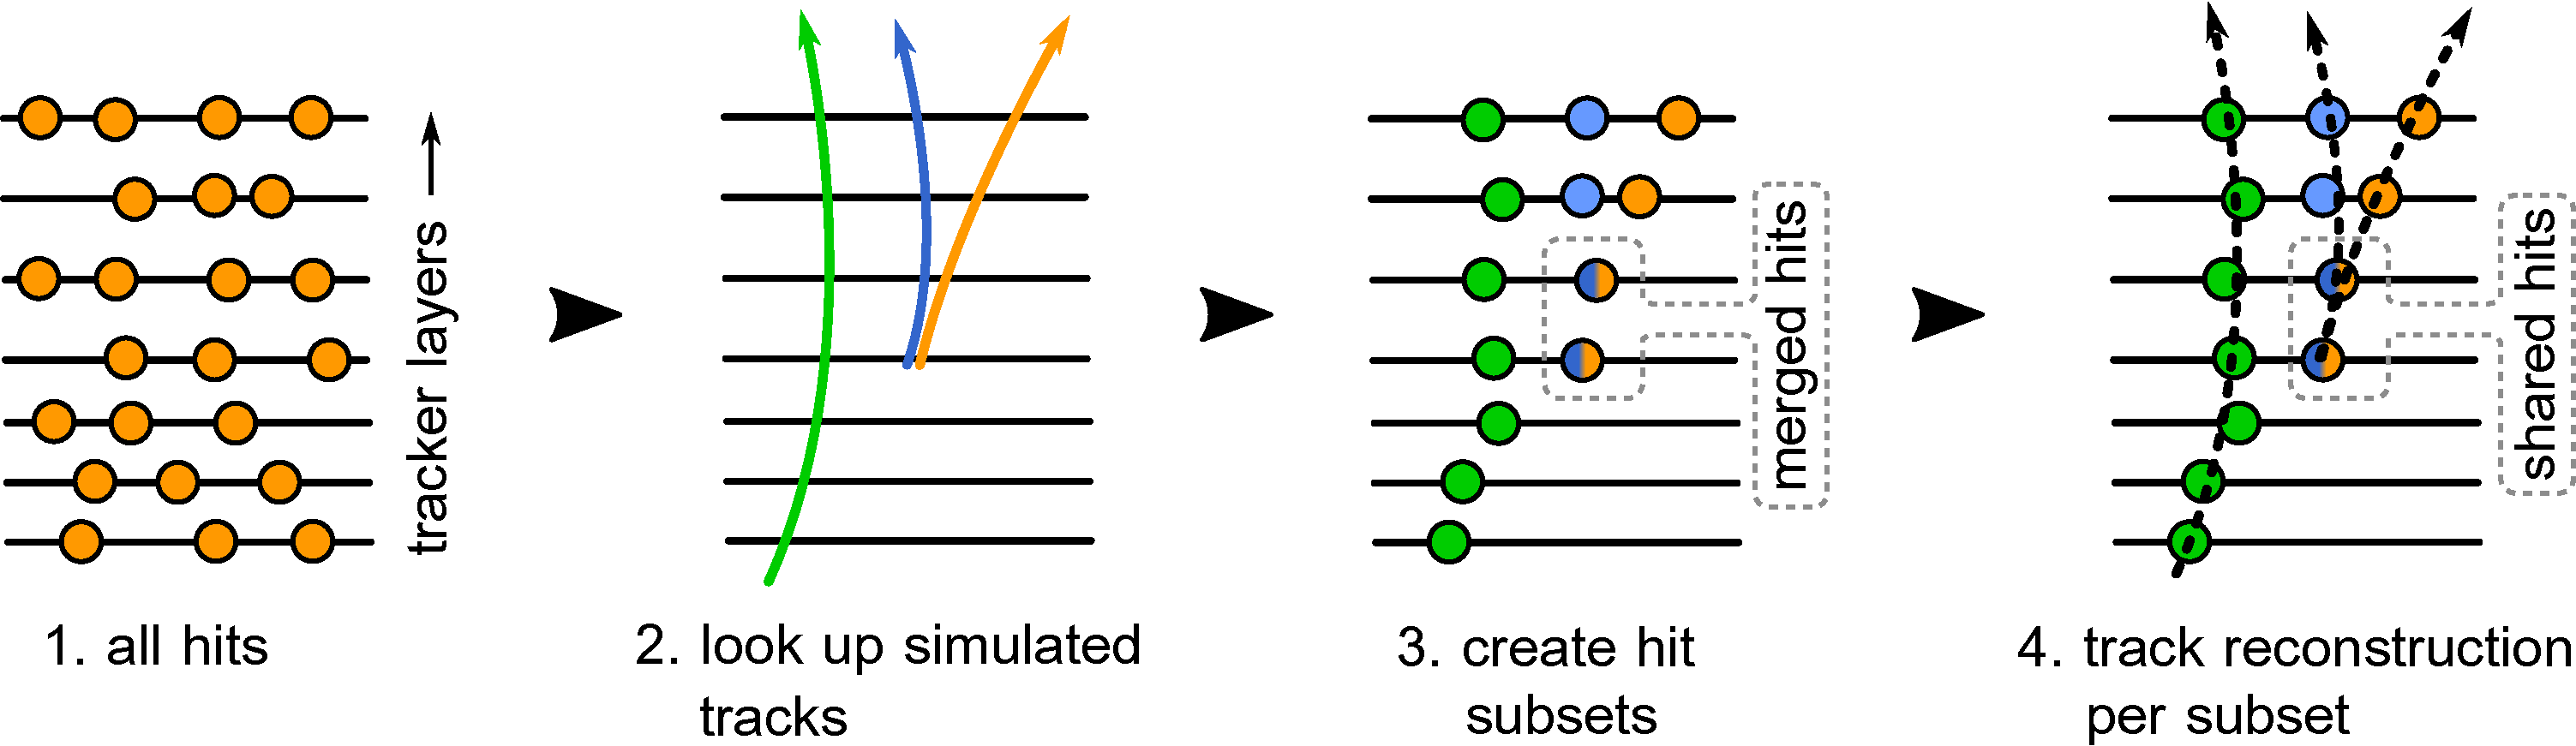
\includegraphics[width=0.95\textwidth]{figures/tracking.pdf}
\caption{\label{fig:tracking}Track reconstruction in \textsc{FastSimulation}. Details are given in the text.}
\end{center}
\end{figure}

The seeding and trajectory building are restricted to the hits within a mapped subset. This removes completely any combinatorial problem from the iterative tracking in \textsc{FastSimulation} resulting in a large reduction of computing time compared to the standard reconstruction. In the seeding step, the acceptance requirements are enforced by interfacing directly with the implemented criteria in the standard seeding step per iteration. The trajectory building process is trivial since the complete set of hits per track has already been defined. Finally, the track is fitted using the standard fit algorithm and the used hits are masked in next iterations.

For the simulation of pileup interactions, additional minimum bias events are first premixed according to the desired pileup scenario and then added to the events at random. In \textsc{FastSimulation}, tracks are already reconstructed in premixed events and then included in the event directly without interfering with the hit and track reconstruction of the main interaction. In analyses, the reconstruction of primary vertices allows to differentiate between tracks stemming from the hard or pileup interactions via their vertex association which motivates this approach.


\section{Validation}

Track reconstruction within \textsc{FastSimulation} is validated by comparing the tracks from the fast emulation with those obtained from the Geant4-based simulation and standard reconstruction. Figure~\ref{fig:eff-tracks} presents the tracking efficiency as a function of the transverse momentum and pseudorapidity. Here, the tracking efficiency is defined as the ratio of reconstructed tracks matched to simulated charged particles over the total number of charged particles within the tracker volume. Furthermore, the obtained resolution of the transverse momentum for reconstructed tracks is shown in Fig.~\ref{fig:res-track}. Overall, the plots demonstrate a good agreement of the \textsc{FastSimulation} tracking performance with the one observed in the Geant4-based simulation and standard reconstruction.

\begin{figure}[!htbp]
\begin{center}
\parbox{0.46\textwidth}{\centering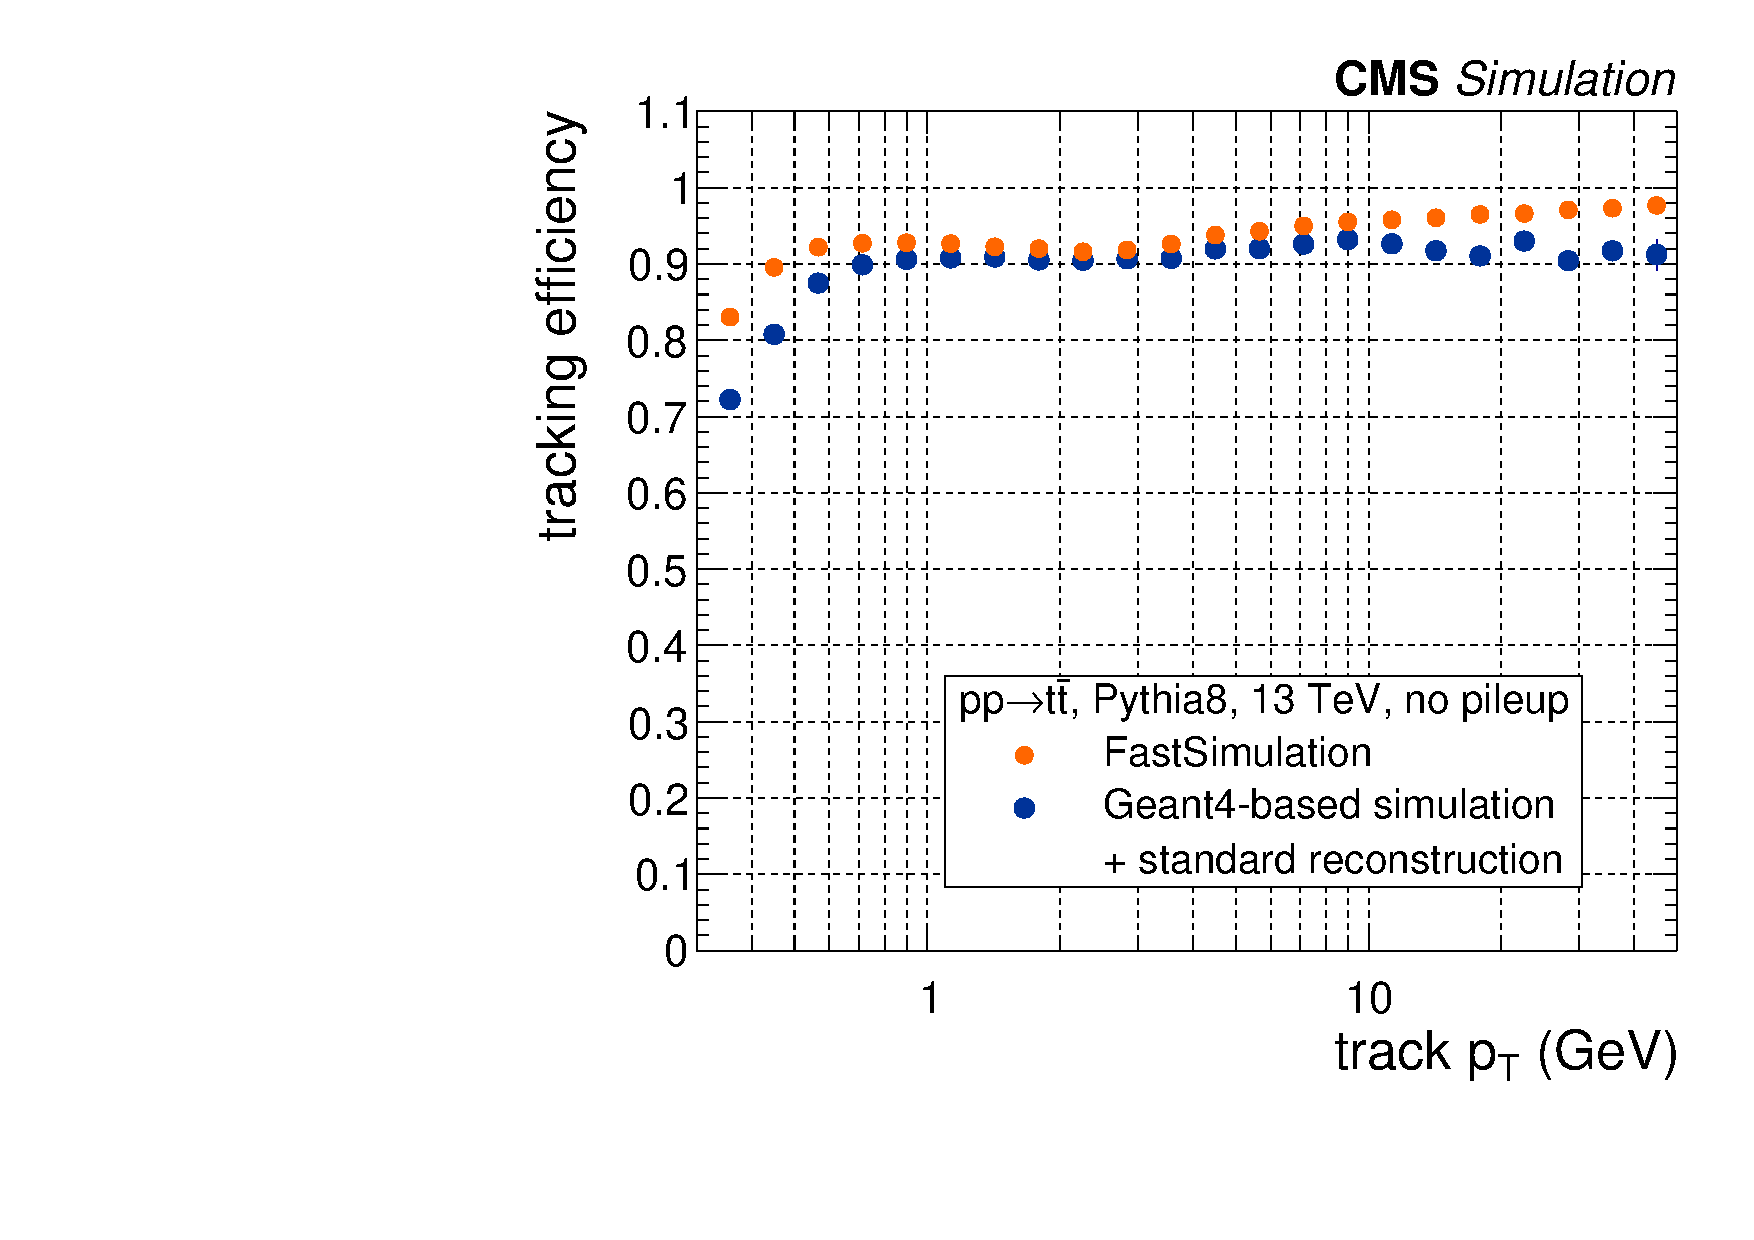
\includegraphics[width=0.45\textwidth]{figures/eff_pt.pdf}\\(a)}
\hspace{0.05\textwidth}
\parbox{0.46\textwidth}{\centering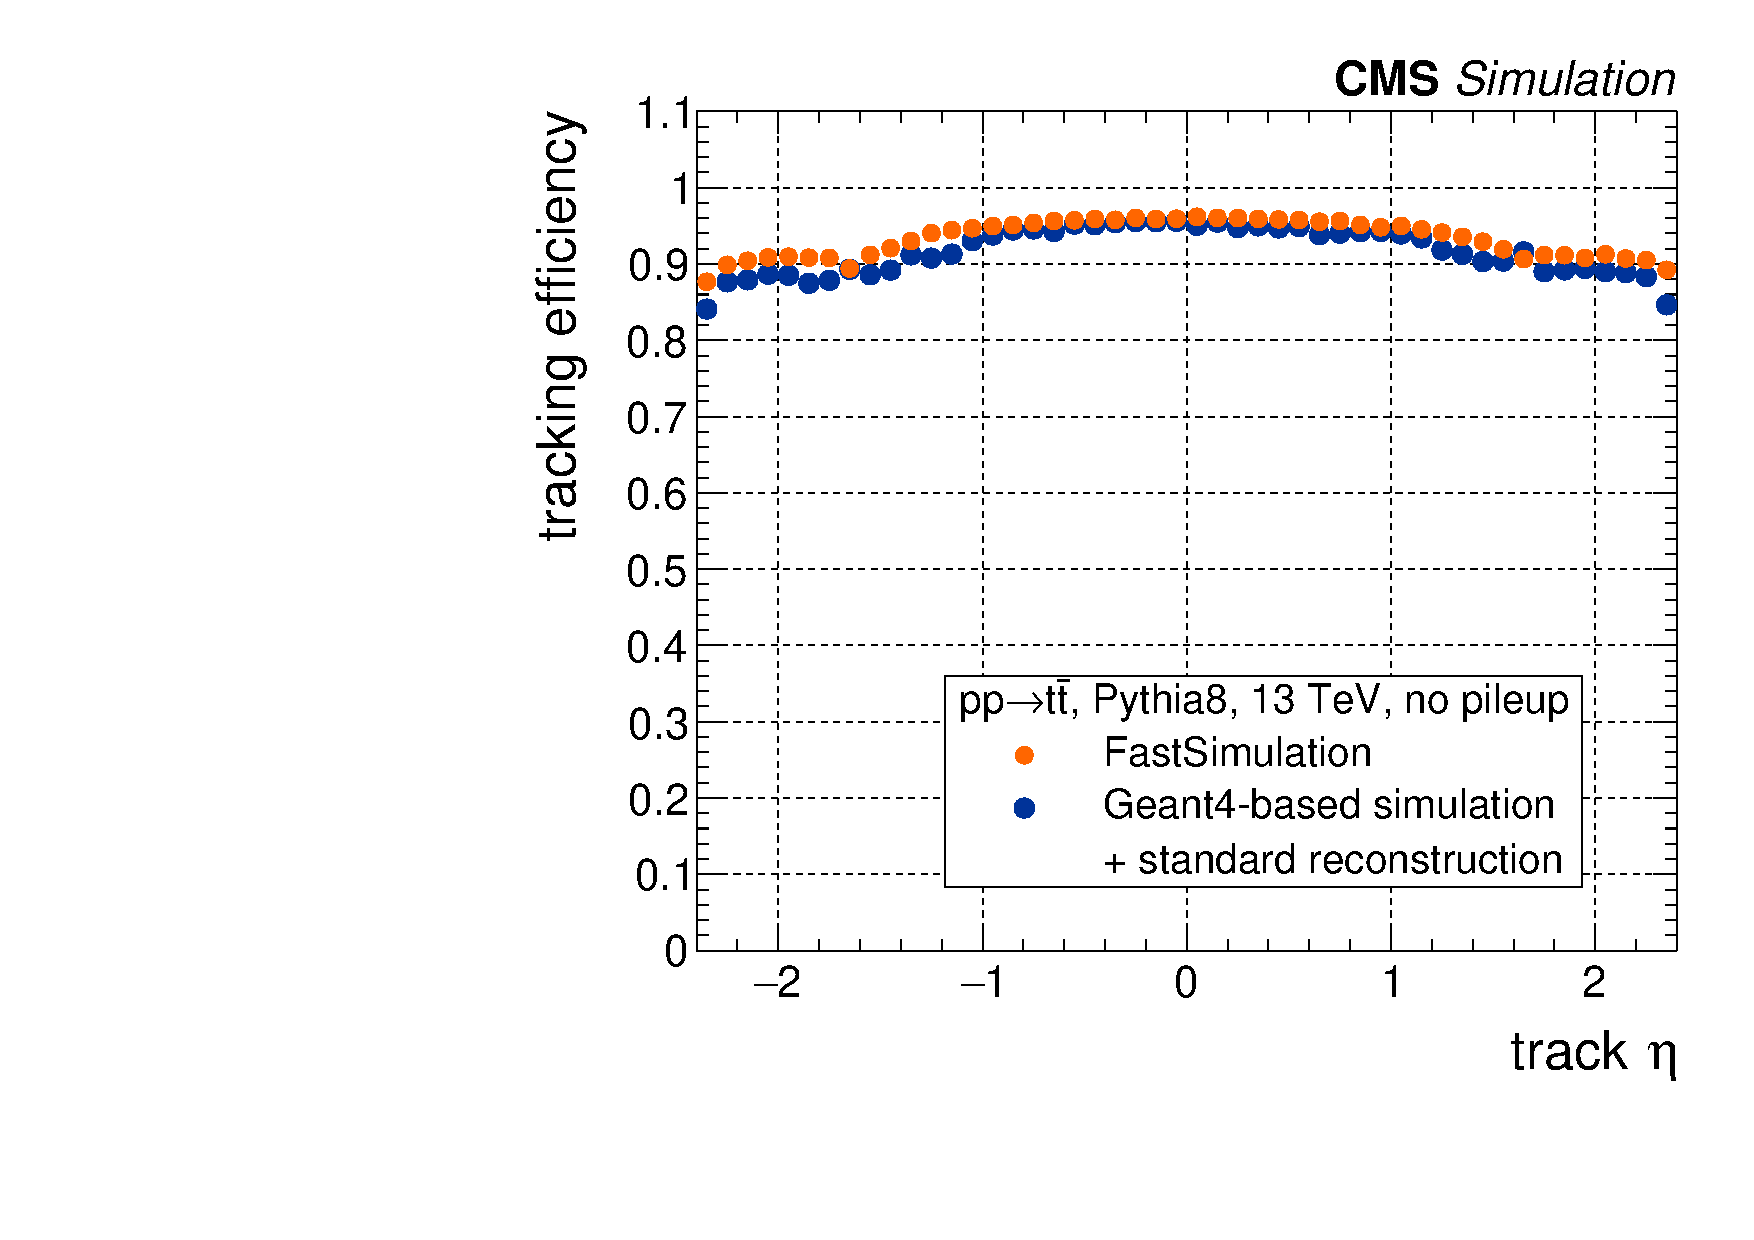
\includegraphics[width=0.45\textwidth]{figures/eff_eta.pdf}\\(b)}
\caption{\label{fig:eff-tracks}Comparison of the reconstruction efficiencies of tracks as a function of (a)~the transverse momentum and (b)~the pseudorapidity measured in the simulation of top quark pair production at 13~TeV.}
\end{center}
\end{figure}



A profile of the average CPU-time consumption per event within \textsc{FastSimulation} is given in Fig.~\ref{fig:cpu} as a function of the average number of pileup interactions. Less than 10~s are required to simulated an event of top quark pair production for current pileup scenarios with $\approx30$ interactions on average. The emulation of tracking is not amongst the top CPU consumers.


\begin{figure}[!htbp]
\begin{center}
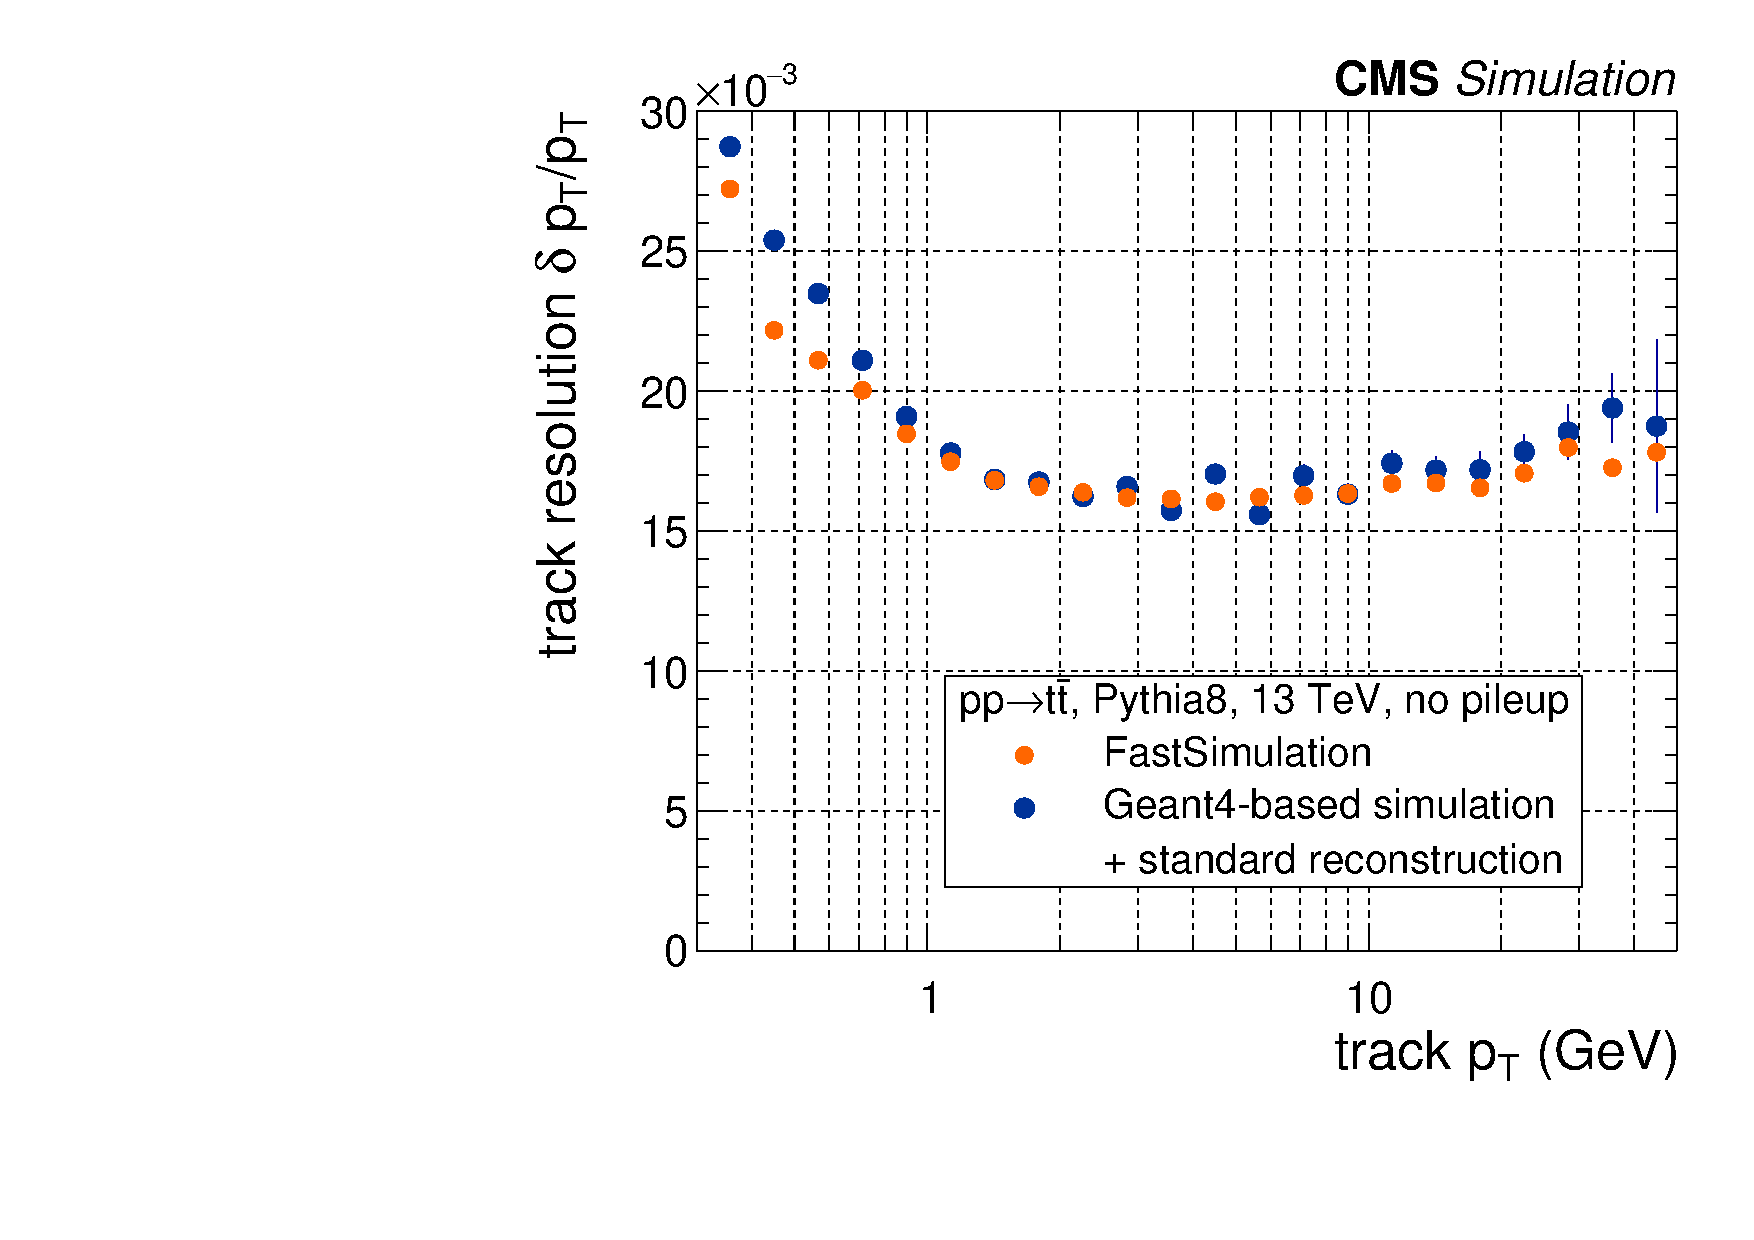
\includegraphics[width=0.45\textwidth]{figures/res_pt.pdf}
\caption{\label{fig:res-track}Comparison of the resolution of reconstructed tracks as a function of the transverse momentum measured in the simulation of top quark pair production at 13~TeV.}
\end{center}
\end{figure}

\clearpage

\begin{figure}[t]
\begin{center}
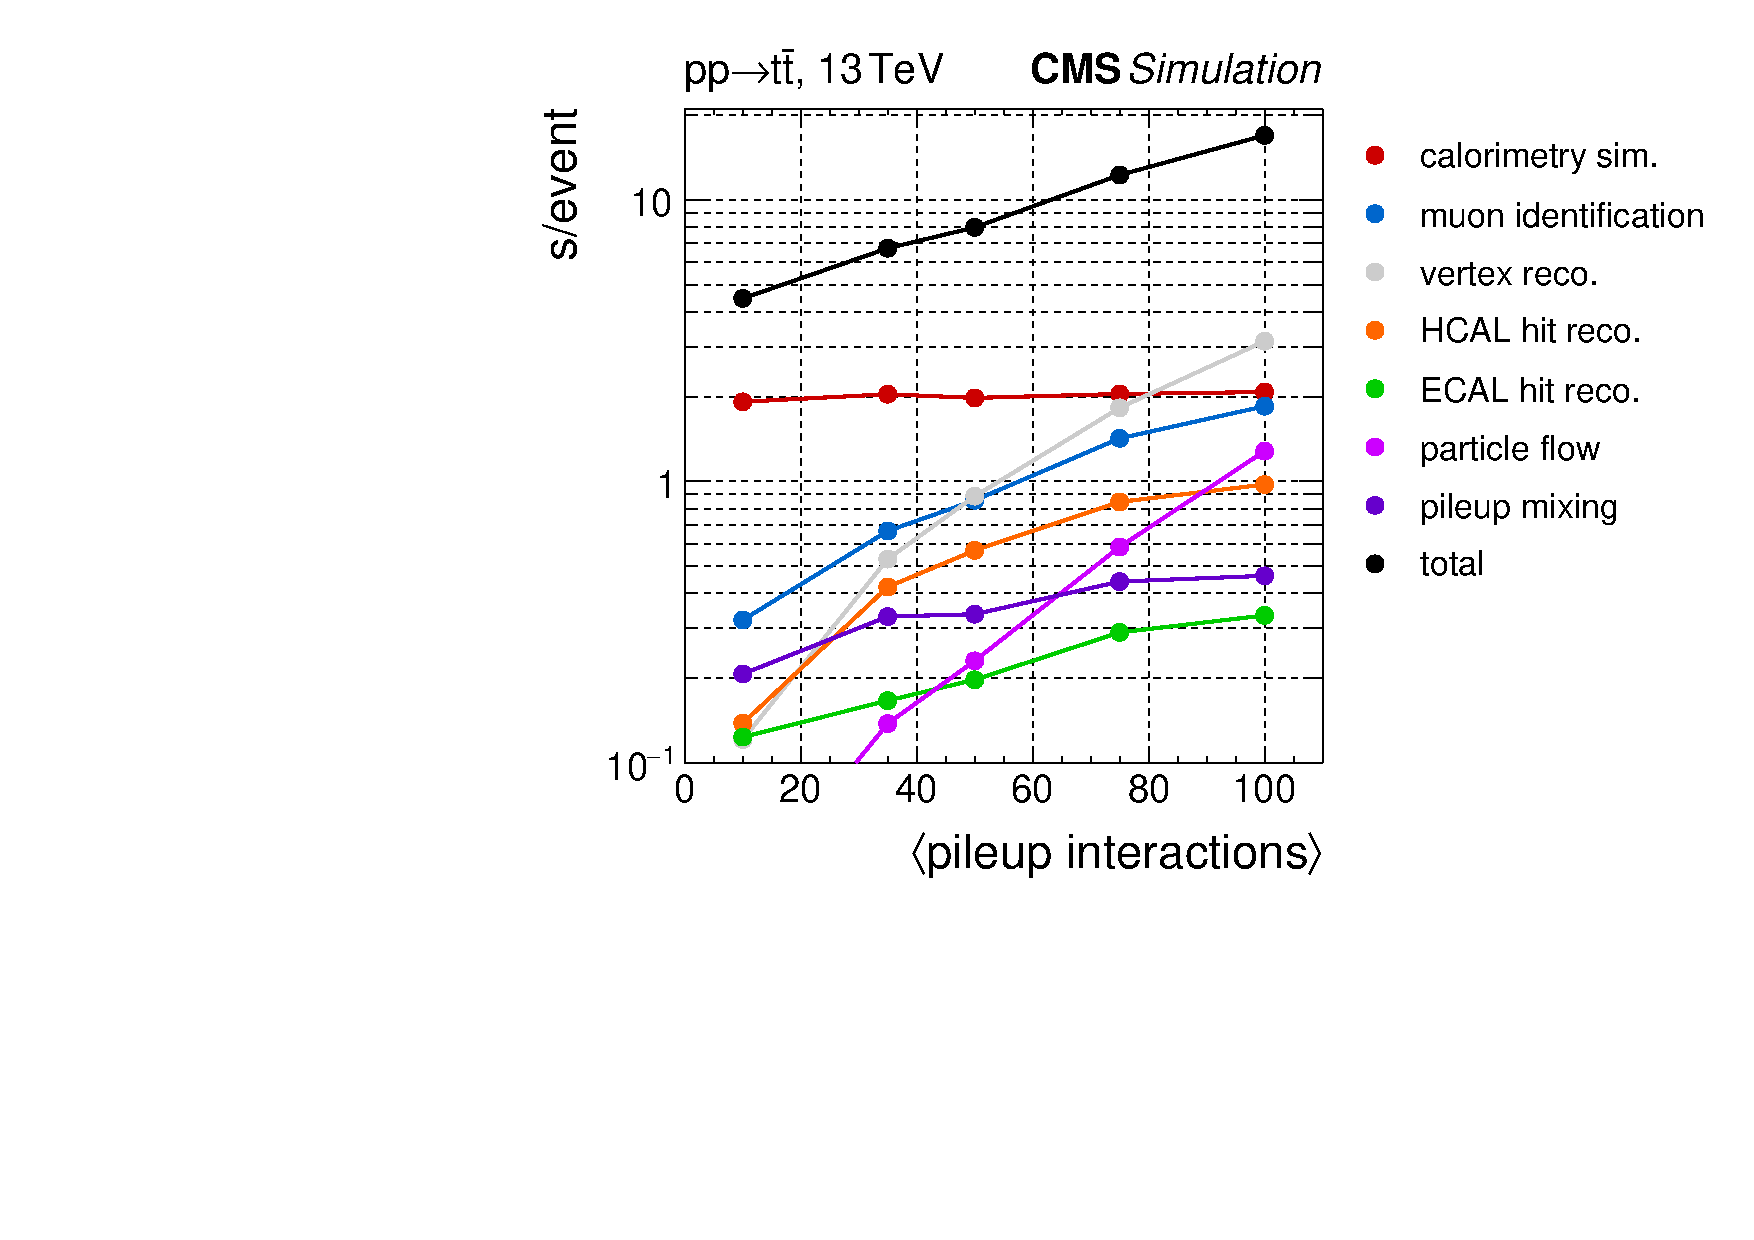
\includegraphics[width=0.55\textwidth]{figures/cpu_profile.pdf}
\caption{\label{fig:cpu}Average CPU-time per event spent on the detector simulation and the reconstruction of analysis objects as a function of the average number of pileup interactions measured in the simulation of top quark pair production at 13~TeV.}
\end{center}
\end{figure}



\section{Conclusion and outlook}

The CMS \textsc{FastSimulation} package provides a fast alternative to the standard simulation and reconstruction workflow. One of its major speedups is the use of truth information in the track reconstruction. Recent developments in the framework led to further flexibility in the emulation of hit reconstruction and to the usage of truth information in the iterative tracking sequence. In the short term, these developments will enable the emulation of the emulation of merged hits originating from close particle tracks. In the long term, the increased flexibility will allow to adapt the emulation of track reconstruction to the planned upgrades of the CMS detector.


\ack
The author thanks the organizers of the \textsc{CHEP2016} conference for the possibility of a poster presentation. Funding is gratefully accepted from Fonds National de Recherche Scientifique~(FNRS), Belgium.



\section*{References}
\begin{thebibliography}{99}
\bibitem{cms} CMS Collaboration 2008 {\it JINST} \textbf{3} S08004.
\bibitem{pf} CMS Collaboration 2009, {\it CMS Physics Analysis Summary} CMS-PAS-PFT-09-001.
\bibitem{fsim1} R. Rahmat et al., 2012, {\it J. Phys. Conf. Ser.} \textbf{396} 062016.
\bibitem{fsim2} A. Giammanco, 2014, {\it J. Phys. Conf. Ser.} \textbf{513} 022012.
\bibitem{cmssw} CMS Collaboration 2006, {\it CMS Technical Design Report} CMS-TDR-8-1.
\bibitem{geant4} S. Agostinelli et al. 2003, {\it Nucl. Instrum. Meth.} A \textbf{506} 250--303. 
\bibitem{pixelav} M. Swartz 2003, {\it Nucl. Instrum. Meth.} A \textbf{511} 88--91.
\bibitem{pixelphase1} CMS Collaboration 2012, {\it CMS Technical Design Report} CMS-TDR-11.
\bibitem{trackreco} CMS Collaboration 2014, {\it JINST} \textbf{9} no.10, P10009.

\end{thebibliography}

\end{document}


